\documentclass[11pt]{article}
\usepackage{mathblatt}
% gesetzt von werkzeuge/setzer.py (Sorte selbst) aus dem Lernweg E69
% und den Bankzeilen; Muster bau/proben/2026-10-09/hypotenuse-muster.
\usepackage{enumitem}
\usepackage{adjustbox,varwidth}
\newgeometry{a4paper,margin=18mm,top=15mm,bottom=20mm,footskip=9mm}
\pagestyle{fancy}\fancyhf{}\renewcommand{\headrulewidth}{0pt}
\fancyfoot[L]{\footnotesize\color{mbgrau}E69 \textperiodcentered{} Kreisfläche}
\fancyfoot[R]{\footnotesize\color{mbgrau}\thepage}
\setlength{\parskip}{3pt}
\renewcommand{\kreuz}[1]{\mbox{$\square$\ #1}\quad}
\newcommand{\kreuzl}[1]{\par\hangindent1.4em\hangafter1\noindent$\square$\ #1}
\newcommand{\aufg}[3]{\par\noindent\makebox[0pt][r]{#3}\begin{minipage}[t]{\linewidth}#1\end{minipage}\par}
\newcommand{\aufgg}[4]{\par\noindent\makebox[0pt][r]{#4}\begin{minipage}[t]{0.6\linewidth}\vspace{0pt}#1\end{minipage}\hfill
  \begin{minipage}[t]{0.37\linewidth}\vspace{0pt}\centering #2\end{minipage}\par}
\newcommand{\nr}[1]{\makebox[7mm][l]{\textbf{#1}}}
\newcommand{\lsg}[3]{\par\noindent\begin{minipage}[t]{9mm}\textbf{#1}\end{minipage}%
  \begin{minipage}[t]{52mm}\raggedright\bfseries\boldmath #2\end{minipage}\hspace{3mm}%
  \begin{minipage}[t]{\dimexpr\linewidth-64mm\relax}\raggedright\small #3\end{minipage}\par\vspace{4pt}}
\newlength{\kr}
\makeatletter
\newcommand{\karomerk}[2]{\protected@write\@auxout{}{\string\karoseite{#1}{#2}{\thepage}}}
\newcommand{\karoseite}[3]{\expandafter\xdef\csname karo@#1@#2\endcsname{#3}}
\newcommand{\karohinweis}[3]{\karomerk{h}{#1}\ifcsname karo@k@#1\endcsname
  \ifnum\csname karo@k@#1\endcsname=0\csname karo@h@#1\endcsname\relax#2\else#3\fi
  \else#3\fi}
\makeatother
\begin{document}

\noindent{\LARGE\bfseries Kreisfläche}\par\smallskip
\noindent{\small\color{mbgrau}Selbstlernheft Klasse 8 \textperiodcentered{} mit Lösungsheft \textperiodcentered{} Kennung E69}\par\medskip
\noindent\textbf{So nutzt du das Heft:} Lies im Abschnitt das Beispiel. Rechne dann die Aufgaben der Reihe nach und vergleiche jede sofort mit dem Lösungsheft. Kreuze „kann ich“ an, wenn du die letzte Aufgabe (\emph{Ziel}) allein schaffst.\par
\noindent Mehr Aufgaben zu einem Abschnitt: Kennung deinem Nachhilfelehrer schicken (z.\,B. „E69 mehr B“).\par\medskip
{\arrayrulecolor{mbgrau}\renewcommand{\arraystretch}{1.3}
\noindent\begin{tabular}{|>{\bfseries}p{10mm}|p{112mm}|>{\raggedleft\arraybackslash}p{10mm}|>{\centering\arraybackslash}p{14mm}|}\hline
\rowcolor{black!8} & \textbf{Abschnitt} & \textbf{Seite} & \textbf{kann ich}\\\hline
A & Fläche aus Radius oder Durchmesser & \pageref{s:A} & $\square$\\\hline
B & Halbkreis und Viertelkreis & \pageref{s:B} & $\square$\\\hline
C & Radius aus der Fläche & \pageref{s:C} & $\square$\\\hline
D & Fläche oder Umfang? & \pageref{s:D} & $\square$\\\hline
T & Probetest & \pageref{s:T} & $\square$\\\hline
\end{tabular}}\par\bigskip

\begin{tcolorbox}[colback=mbkasten,colframe=mbgrau,boxrule=0.5pt,arc=1mm,left=3mm,right=3mm,top=2mm,bottom=2mm,title={\bfseries Formel auf einen Blick},coltitle=black,colbacktitle=black!10]
\begin{minipage}[t]{0.58\linewidth}\vspace{0pt}
{\Large $A = \pi \cdot r^2$ \qquad $r = d : 2$}\par\medskip
In Worten: Die Fläche ist $\pi$ mal Radius mal Radius. Ist der Durchmesser gegeben, erst halbieren.\par\medskip
\textbf{So gehst du vor}\par
\nr{1}Radius oder Durchmesser? Ist es $d$, halbieren\par
\nr{2}$A = \pi \cdot r^2$ mit der Taste $\pi$\par
\nr{3}erst am Ende runden, Einheit cm² oder m²\par
\nr{4}rückwärts: $r^2 = A : \pi$, dann die Wurzel\par
\medskip
{\small Rechne mit der Taste $\pi$ und runde erst am Ende – auf eine Stelle nach dem Komma, wenn nichts anderes steht.}
\end{minipage}\hfill
\begin{minipage}[t]{0.38\linewidth}\vspace{2mm}\centering
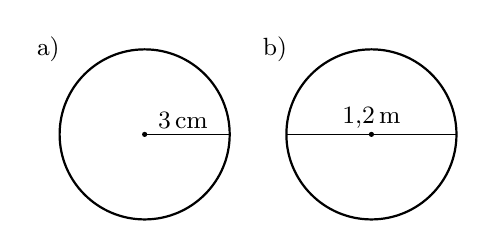
\begin{tikzpicture}[scale=0.72,font=\small]\draw[line width=0.8pt] (0,0) circle (1.5);\fill (0,0) circle (1.3pt);\draw[line width=0.6pt] (0,0) -- (1.500,0.000);\node[anchor=south,inner sep=2pt] at (0.675,0.000) {3\,cm};\node[font=\small] at (-1.7,1.5) {a)};\draw[line width=0.8pt] (4.0,0) circle (1.5);\fill (4.0,0) circle (1.3pt);\draw[line width=0.6pt] (2.5,0) -- (5.5,0);\node[anchor=south,inner sep=2pt] at (4.0,0) {1{,}2\,m};\node[font=\small] at (2.3,1.5) {b)};\end{tikzpicture}
\end{minipage}
\end{tcolorbox}
\medskip\noindent\textbf{Typische Fehler – so nicht}\par\smallskip
\noindent\nr{$\times$}Durchmesser eingesetzt: bei $d = 8$\,cm ist $r = 4$\,cm, nicht 8\,cm.\par
\noindent\nr{$\times$}$r^2$ als $2 \cdot r$ gerechnet: $5^2 = 25$, nicht 10.\par
\noindent\nr{$\times$}Umfang und Fläche vertauscht: Rand ist $u$ (cm), innen ist $A$ (cm²).\par
\noindent\nr{$\times$}Beim Rückwärtsrechnen die Wurzel vergessen: $A : \pi$ ist erst $r^2$.\par
\clearpage\label{s:A}\noindent\colorbox{black!12}{\makebox[10mm]{\Large\bfseries\strut A}}\hspace{3mm}{\Large\bfseries Fläche aus Radius oder Durchmesser}\par\smallskip
\noindent Die Fläche ist $\pi$ mal Radius mal Radius. Der Radius $r$ geht vom Mittelpunkt bis zum Rand, der Durchmesser $d$ ganz hindurch und ist doppelt so lang. Ist $d$ gegeben, halbierst du zuerst.\par\medskip
\noindent\textbf{Formel}\par\nopagebreak\noindent\hspace*{4mm}\begin{minipage}{\dimexpr\linewidth-4mm\relax}$A = \pi \cdot r^2 = \pi \cdot r \cdot r$ \qquad $r = d : 2$ \qquad {\small ($\pi \approx 3{,}14$, nimm die Taste $\pi$)}\end{minipage}\par\medskip
\noindent\textbf{Beispiel}\quad (a) Berechne die Fläche des Kreises mit $r = 3$\,cm. (b) Ein runder Tisch hat 1,2\,m Durchmesser. Ein Topf Lack reicht für 1\,m². Reicht er für die Tischplatte?\par\smallskip
\noindent\begin{minipage}[t]{0.6\linewidth}\vspace{0pt}\par\noindent\hangindent6mm\hangafter1\makebox[6mm][l]{\textbf{1}}(a) Gegeben ist der Radius (vom Mittelpunkt zum Rand): $r = 3$\,cm.\par\smallskip\par\noindent\hangindent6mm\hangafter1\makebox[6mm][l]{\textbf{2}}$A = \pi \cdot 3^2 = \pi \cdot 9$. Tippe $\pi \cdot 9$ in den Taschenrechner: $28{,}274\ldots$ Erst jetzt runden: $A \approx 28{,}3$\,cm².\par\smallskip\par\noindent\hangindent6mm\hangafter1\makebox[6mm][l]{\textbf{3}}(b) Gegeben ist der Durchmesser. Erst halbieren: $r = 1{,}2 : 2 = 0{,}6$\,m.\par\smallskip\par\noindent\hangindent6mm\hangafter1\makebox[6mm][l]{\textbf{4}}$A = \pi \cdot 0{,}6^2 = \pi \cdot 0{,}36 \approx 1{,}13$\,m² (auf zwei Stellen, damit man den Unterschied sieht).\par\smallskip\par\noindent\hangindent6mm\hangafter1\makebox[6mm][l]{\textbf{5}}Vergleichen: $1{,}13 > 1$. Der Lack reicht nicht, es fehlen etwa $0{,}13$\,m².\par\smallskip\end{minipage}\hfill
\begin{minipage}[t]{0.37\linewidth}\vspace{0pt}\centering 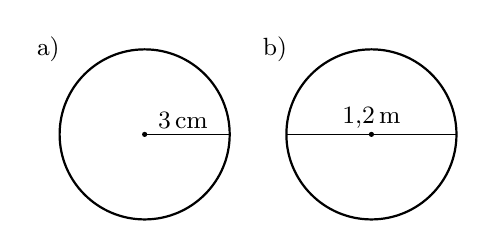
\begin{tikzpicture}[scale=0.72,font=\small]\draw[line width=0.8pt] (0,0) circle (1.5);\fill (0,0) circle (1.3pt);\draw[line width=0.6pt] (0,0) -- (1.500,0.000);\node[anchor=south,inner sep=2pt] at (0.675,0.000) {3\,cm};\node[font=\small] at (-1.7,1.5) {a)};\draw[line width=0.8pt] (4.0,0) circle (1.5);\fill (4.0,0) circle (1.3pt);\draw[line width=0.6pt] (2.5,0) -- (5.5,0);\node[anchor=south,inner sep=2pt] at (4.0,0) {1{,}2\,m};\node[font=\small] at (2.3,1.5) {b)};\end{tikzpicture}\end{minipage}\par\medskip
\noindent\textbf{Aufgaben}\hspace{1em}{\small\color{mbgrau}\karohinweis{A}{Rechne unten im Karo.}{Rechne auf einem extra Blatt.} Vergleiche jede Aufgabe gleich mit dem Lösungsheft.}\par\smallskip
\aufg{\hangindent7mm\hangafter1\nr{1.}Berechne die Fläche des Kreises. (a) $r = 5$\,cm\quad (b) $r = 10$\,cm\quad (c) $r = 4$\,m}{}{}
\medskip
\aufgg{\hangindent7mm\hangafter1\nr{2.}Radius oder Durchmesser? Berechne die Fläche.}{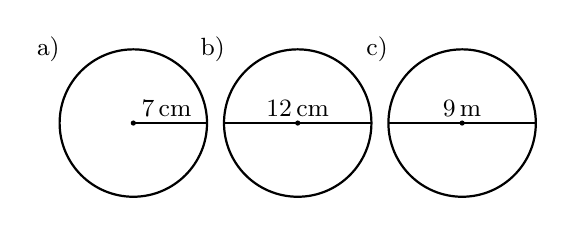
\begin{tikzpicture}[scale=0.72,font=\small]\draw[line width=0.8pt] (0,0) circle (1.3);\fill (0,0) circle (1.3pt);\draw[line width=0.6pt] (0,0) -- (1.300,0.000);\node[anchor=south,inner sep=2pt] at (0.585,0.000) {7\,cm};\node[font=\small] at (-1.5,1.3) {a)};\draw[line width=0.8pt] (2.9,0) circle (1.3);\fill (2.9,0) circle (1.3pt);\draw[line width=0.6pt] (1.5999999999999999,0) -- (4.2,0);\node[anchor=south,inner sep=2pt] at (2.9,0) {12\,cm};\node[font=\small] at (1.4,1.3) {b)};\draw[line width=0.8pt] (5.8,0) circle (1.3);\fill (5.8,0) circle (1.3pt);\draw[line width=0.6pt] (4.5,0) -- (7.1,0);\node[anchor=south,inner sep=2pt] at (5.8,0) {9\,m};\node[font=\small] at (4.3,1.3) {c)};\end{tikzpicture}}{}{}
\medskip
\aufg{\hangindent7mm\hangafter1\nr{3.}Berechne die Fläche. Runde auf zwei Stellen nach dem Komma. (a) $r = 2{,}5$\,cm\quad (b) $d = 1{,}8$\,m}{}{}
\medskip
\aufg{\hangindent7mm\hangafter1\nr{4.}In der Pizzeria gibt es runde Pizzen: groß mit 32\,cm Durchmesser, klein mit 22\,cm Durchmesser. Lena überlegt: eine große oder zwei kleine? Wobei bekommt sie mehr Pizza? Um wie viel? Runde auf ganze cm².}{}{{\scriptsize\color{mbgrau}Ziel\hspace{2mm}}}
\medskip
\par\vspace{3mm}\setlength{\kr}{\dimexpr\pagegoal-\pagetotal-10mm\relax}%
\ifdim\kr>12mm\karomerk{k}{A}\noindent{\scriptsize\color{mbgrau}Platz zum Rechnen}\par\nointerlineskip\vspace{1mm}\noindent
\begin{tikzpicture}\clip (0,0) rectangle ({\linewidth-0.5mm},\kr);\draw[black!16,line width=0.3pt,step=5mm] (0,0) grid (\linewidth,\kr);\end{tikzpicture}\fi\par
\clearpage\label{s:B}\noindent\colorbox{black!12}{\makebox[10mm]{\Large\bfseries\strut B}}\hspace{3mm}{\Large\bfseries Halbkreis und Viertelkreis}\par\smallskip
\noindent Ein Halbkreis ist die Hälfte der Kreisfläche, ein Viertelkreis ein Viertel. Rechne den ganzen Kreis mit demselben Radius und teile durch 2 oder durch 4.\par\medskip
\noindent\textbf{Formel}\par\nopagebreak\noindent\hspace*{4mm}\begin{minipage}{\dimexpr\linewidth-4mm\relax}Halbkreis: $A = \pi \cdot r^2 : 2$ \qquad Viertelkreis: $A = \pi \cdot r^2 : 4$\end{minipage}\par\medskip
\noindent\textbf{Beispiel}\quad (a) Berechne die Fläche des Halbkreises. (b) Ein Rasensprenger steht in der Ecke eines Gartens und spritzt 6\,m weit. Wie groß ist die Fläche, die er nass macht?\par\smallskip
\noindent\begin{minipage}[t]{0.6\linewidth}\vspace{0pt}\par\noindent\hangindent6mm\hangafter1\makebox[6mm][l]{\textbf{1}}(a) Die gerade Seite des Halbkreises ist der Durchmesser. Erst halbieren: $r = 10 : 2 = 5$\,cm.\par\smallskip\par\noindent\hangindent6mm\hangafter1\makebox[6mm][l]{\textbf{2}}Ganzer Kreis mit diesem Radius, dann die Hälfte: $A = \pi \cdot 5^2 : 2 = 39{,}26\ldots \approx 39{,}3$\,cm².\par\smallskip\par\noindent\hangindent6mm\hangafter1\makebox[6mm][l]{\textbf{3}}(b) Der Sprenger erreicht alles bis 6\,m: Das ist ein Kreis mit $r = 6$\,m. Die Ecke ist ein rechter Winkel, darum liegt nur ein Viertel des Kreises im Garten. Skizze: zwei Radien mit rechtem Winkel, dazwischen der Bogen.\par\smallskip\par\noindent\hangindent6mm\hangafter1\makebox[6mm][l]{\textbf{4}}$A = \pi \cdot 6^2 : 4 = \pi \cdot 36 : 4 \approx 28{,}3$\,m².\par\smallskip\par\noindent\hangindent6mm\hangafter1\makebox[6mm][l]{\textbf{5}}Merke: Zwei gleiche Halbkreise sind zusammen ein ganzer Kreis. Gehört noch ein Rechteck dazu, rechne es extra und zähle die Flächen zusammen.\par\smallskip\end{minipage}\hfill
\begin{minipage}[t]{0.37\linewidth}\vspace{0pt}\centering 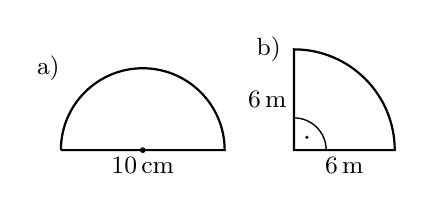
\begin{tikzpicture}[scale=0.8,font=\small]\draw[line width=0.8pt] (-1.3,0) -- (1.3,0) arc (0:180:1.3);\fill (0,0) circle (1.3pt);\node[anchor=north,inner sep=2.5pt] at (0,0) {10\,cm};\node[font=\small] at (-1.5,1.3) {a)};\draw[line width=0.8pt] (2.4,0) -- (4.0,0) arc (0:90:1.6) -- cycle;\draw[line width=0.5pt] (2.912,0) arc (0:90:0.512);\fill (2.6048,0.2048) circle (0.8pt);\node[anchor=north,inner sep=2.5pt] at (3.2,0) {6\,m};\node[anchor=east,inner sep=2.5pt] at (2.4,0.8) {6\,m};\node[font=\small] at (2.0,1.6) {b)};\end{tikzpicture}\end{minipage}\par\medskip
\noindent\textbf{Aufgaben}\hspace{1em}{\small\color{mbgrau}\karohinweis{B}{Rechne unten im Karo.}{Rechne auf einem extra Blatt.} Vergleiche jede Aufgabe gleich mit dem Lösungsheft.}\par\smallskip
\aufgg{\hangindent7mm\hangafter1\nr{1.}Berechne die Fläche der Figur.}{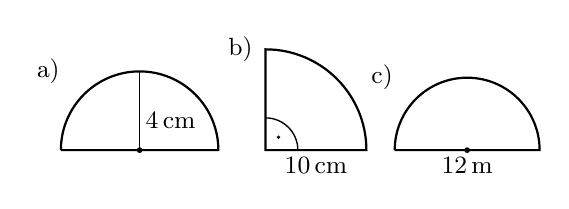
\begin{tikzpicture}[scale=0.8,font=\small]\draw[line width=0.8pt] (-1.25,0) -- (1.25,0) arc (0:180:1.25);\fill (0,0) circle (1.3pt);\draw[line width=0.6pt] (0,0) -- (0,1.25);\node[anchor=west,inner sep=2pt] at (0,0.475) {4\,cm};\node[font=\small] at (-1.45,1.25) {a)};\draw[line width=0.8pt] (2.0,0) -- (3.6,0) arc (0:90:1.6) -- cycle;\draw[line width=0.5pt] (2.512,0) arc (0:90:0.512);\fill (2.2048,0.2048) circle (0.8pt);\node[anchor=north,inner sep=2.5pt] at (2.8,0) {10\,cm};\node[font=\small] at (1.6,1.6) {b)};\draw[line width=0.8pt] (4.050000000000001,0) -- (6.35,0) arc (0:180:1.15);\fill (5.2,0) circle (1.3pt);\node[anchor=north,inner sep=2.5pt] at (5.2,0) {12\,m};\node[font=\small] at (3.8500000000000005,1.15) {c)};\end{tikzpicture}}{}{}
\medskip
\aufgg{\hangindent7mm\hangafter1\nr{2.}Der Viertelkreis hat den Radius $a$. Welcher Term gibt seine Fläche an? Kreuze an. Rechne ihn dann für $a = 8$\,cm aus.\par\smallskip\leftskip7mm \kreuz{$\pi \cdot a^2 : 2$}\ \kreuz{$\pi \cdot a^2 : 4$}\par\kreuz{$2 \cdot \pi \cdot a : 4$}\ \kreuz{$\pi \cdot (a : 4)^2$}}{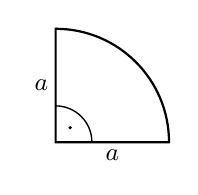
\begin{tikzpicture}[scale=0.8,font=\small]\draw[line width=0.8pt] (0,0) -- (1.8,0) arc (0:90:1.8) -- cycle;\draw[line width=0.5pt] (0.5760000000000001,0) arc (0:90:0.5760000000000001);\fill (0.23040000000000005,0.23040000000000005) circle (0.8pt);\node[anchor=north,inner sep=2.5pt] at (0.9,0) {$a$};\node[anchor=east,inner sep=2.5pt] at (0,0.9) {$a$};\end{tikzpicture}}{}{}
\medskip
\aufgg{\hangindent7mm\hangafter1\nr{3.}Ein Sportplatz besteht aus einem Rechteck und zwei Halbkreisen. (a) Wie groß sind die beiden Halbkreise zusammen? (b) Wie groß ist der ganze Platz?}{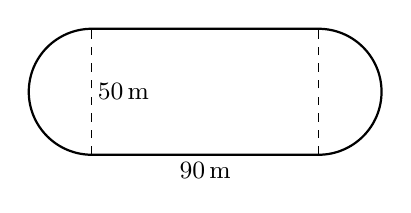
\begin{tikzpicture}[scale=0.8,font=\small]\draw[line width=0.8pt] (0,0) -- (3.6,0) arc (-90:90:1) -- (0,2) arc (90:270:1);\draw[dashed,line width=0.5pt] (0,0) -- (0,2);\draw[dashed,line width=0.5pt] (3.6,0) -- (3.6,2);\node[anchor=north,inner sep=2.5pt] at (1.8,0) {90\,m};\node[anchor=west,inner sep=2pt] at (0,1) {50\,m};\end{tikzpicture}}{}{}
\medskip
\aufg{\hangindent7mm\hangafter1\nr{4.}Ein Rasensprenger steht an einer langen, geraden Hecke, genau in der Mitte. Er spritzt 5\,m weit und dreht sich nur auf der Rasenseite. Eine Tüte Rasensamen reicht für 35\,m². Reicht eine Tüte für die Fläche, die er nass macht? Begründe mit einer Rechnung.}{}{{\scriptsize\color{mbgrau}Ziel\hspace{2mm}}}
\medskip
\par\vspace{3mm}\setlength{\kr}{\dimexpr\pagegoal-\pagetotal-10mm\relax}%
\ifdim\kr>12mm\karomerk{k}{B}\noindent{\scriptsize\color{mbgrau}Platz zum Rechnen}\par\nointerlineskip\vspace{1mm}\noindent
\begin{tikzpicture}\clip (0,0) rectangle ({\linewidth-0.5mm},\kr);\draw[black!16,line width=0.3pt,step=5mm] (0,0) grid (\linewidth,\kr);\end{tikzpicture}\fi\par
\clearpage\label{s:C}\noindent\colorbox{black!12}{\makebox[10mm]{\Large\bfseries\strut C}}\hspace{3mm}{\Large\bfseries Radius aus der Fläche}\par\smallskip
\noindent Kennst du die Fläche, rechnest du rückwärts: erst durch $\pi$ teilen, dann die Wurzel ziehen. Das ist der Radius; der Durchmesser ist doppelt so lang.\par\medskip
\noindent\textbf{Formel}\par\nopagebreak\noindent\hspace*{4mm}\begin{minipage}{\dimexpr\linewidth-4mm\relax}$r^2 = A : \pi$ \qquad $r = \sqrt{A : \pi}$ \qquad $d = 2 \cdot r$\end{minipage}\par\medskip
\noindent\textbf{Beispiel}\quad Ein Kreis hat die Fläche 154\,cm². Wie lang sind Radius und Durchmesser?\par\smallskip
\noindent\par\noindent\hangindent6mm\hangafter1\makebox[6mm][l]{\textbf{1}}Formel aufschreiben und die Fläche einsetzen: $\pi \cdot r^2 = 154$.\par\smallskip\par\noindent\hangindent6mm\hangafter1\makebox[6mm][l]{\textbf{2}}Durch $\pi$ teilen: $r^2 = 154 : \pi = 49{,}01\ldots$ Nicht runden, mit dem Wert im Rechner weiter.\par\smallskip\par\noindent\hangindent6mm\hangafter1\makebox[6mm][l]{\textbf{3}}Wurzel ziehen: $r = \sqrt{49{,}01\ldots} \approx 7{,}0$\,cm. Achtung: $49{,}01$ ist erst $r^2$, noch nicht $r$.\par\smallskip\par\noindent\hangindent6mm\hangafter1\makebox[6mm][l]{\textbf{4}}Durchmesser: $d = 2 \cdot r \approx 14{,}0$\,cm.\par\smallskip\par\noindent\hangindent6mm\hangafter1\makebox[6mm][l]{\textbf{5}}Probe: $\pi \cdot 7^2 \approx 153{,}9 \approx 154$. Passt.\par\smallskip\par\medskip
\noindent\textbf{Aufgaben}\hspace{1em}{\small\color{mbgrau}\karohinweis{C}{Rechne unten im Karo.}{Rechne auf einem extra Blatt.} Vergleiche jede Aufgabe gleich mit dem Lösungsheft.}\par\smallskip
\aufg{\hangindent7mm\hangafter1\nr{1.}Berechne den Radius. (a) $A = 314$\,cm²\quad (b) $A = 78{,}5$\,m²\quad (c) $A = 12{,}6$\,cm²}{}{}
\medskip
\aufg{\hangindent7mm\hangafter1\nr{2.}Berechne den Durchmesser. (a) $A = 50$\,cm²\quad (b) $A = 2$\,m²}{}{}
\medskip
\aufg{\hangindent7mm\hangafter1\nr{3.}Ein rundes Sonnensegel soll 12\,m² Schatten geben. Welchen Durchmesser muss es haben? Runde auf zwei Stellen.}{}{}
\medskip
\aufg{\hangindent7mm\hangafter1\nr{4.}Eine Ziege wird mit einem Strick an einen Pflock auf der Wiese gebunden. Sie soll mindestens 45\,m² Gras zum Fressen haben. Im Schuppen liegen Stricke mit 3\,m, 4\,m und 5\,m Länge. Welches ist der kürzeste Strick, der reicht? Kreuze an.\par\smallskip\leftskip7mm \kreuz{3\,m}\ \kreuz{4\,m}\par\kreuz{5\,m}}{}{{\scriptsize\color{mbgrau}Ziel\hspace{2mm}}}
\medskip
\par\vspace{3mm}\setlength{\kr}{\dimexpr\pagegoal-\pagetotal-10mm\relax}%
\ifdim\kr>12mm\karomerk{k}{C}\noindent{\scriptsize\color{mbgrau}Platz zum Rechnen}\par\nointerlineskip\vspace{1mm}\noindent
\begin{tikzpicture}\clip (0,0) rectangle ({\linewidth-0.5mm},\kr);\draw[black!16,line width=0.3pt,step=5mm] (0,0) grid (\linewidth,\kr);\end{tikzpicture}\fi\par
\clearpage\label{s:D}\noindent\colorbox{black!12}{\makebox[10mm]{\Large\bfseries\strut D}}\hspace{3mm}{\Large\bfseries Fläche oder Umfang?}\par\smallskip
\noindent Die Fläche liegt innen (Rasen, Folie, Stoff), in cm² oder m². Der Umfang ist der Rand einmal herum (Zaun, Borte, ein Rad rollt einmal ab), in cm oder m. Lies zuerst, was gefragt ist.\par\medskip
\noindent\textbf{Formel}\par\nopagebreak\noindent\hspace*{4mm}\begin{minipage}{\dimexpr\linewidth-4mm\relax}Fläche: $A = \pi \cdot r^2$ \qquad Umfang: $u = \pi \cdot d = 2 \cdot \pi \cdot r$\end{minipage}\par\medskip
\noindent\textbf{Beispiel}\quad Ein rundes Beet hat 6\,m Durchmesser. (a) Um das Beet kommen Kantensteine. Wie lang ist der Rand? (b) Wie groß ist die Fläche zum Bepflanzen? (c) Ein Kantenstein ist 40\,cm lang. Wie viele Steine braucht man?\par\smallskip
\noindent\par\noindent\hangindent6mm\hangafter1\makebox[6mm][l]{\textbf{1}}(a) Kantensteine liegen am Rand: gefragt ist der Umfang, Einheit m. $u = \pi \cdot d = \pi \cdot 6 \approx 18{,}8$\,m. Der Umfang ist gut dreimal so lang wie der Durchmesser.\par\smallskip\par\noindent\hangindent6mm\hangafter1\makebox[6mm][l]{\textbf{2}}(b) Bepflanzen: gefragt ist die Fläche innen, Einheit m². Erst $r = 6 : 2 = 3$\,m, dann $A = \pi \cdot 3^2 \approx 28{,}3$\,m².\par\smallskip\par\noindent\hangindent6mm\hangafter1\makebox[6mm][l]{\textbf{3}}(c) Gleiche Einheit: 40\,cm $= 0{,}4$\,m. $18{,}85 : 0{,}4 = 47{,}1\ldots$\par\smallskip\par\noindent\hangindent6mm\hangafter1\makebox[6mm][l]{\textbf{4}}47 Steine reichen nicht ganz, darum aufrunden: 48 Steine.\par\smallskip\par\medskip
\noindent\textbf{Aufgaben}\hspace{1em}{\small\color{mbgrau}\karohinweis{D}{Rechne unten im Karo.}{Rechne auf einem extra Blatt.} Vergleiche jede Aufgabe gleich mit dem Lösungsheft.}\par\smallskip
\aufg{\hangindent7mm\hangafter1\nr{1.}Fläche oder Umfang? Schreib F oder U. (a) Zaun um einen runden Teich\quad (b) Folie für den Teichboden\quad (c) Borte am Rand einer runden Tischdecke\quad (d) Farbe für ein rundes Schild\quad (e) Weg, den ein Rad bei einer Umdrehung rollt}{}{}
\medskip
\aufg{\hangindent7mm\hangafter1\nr{2.}Ergänze die Tabelle.\adjustbox{max width=\linewidth}{\begin{varwidth}{50cm}\sachtabelle{lcccc}{ & $r$ & $d$ & $u$ & $A$}{(a) & 5\,cm & \leerzelle & \leerzelle & \leerzelle\\ (b) & \leerzelle & 8\,m & \leerzelle & \leerzelle\\ (c) & 1{,}5\,cm & \leerzelle & \leerzelle & \leerzelle}\end{varwidth}}}{}{}
\medskip
\aufg{\hangindent7mm\hangafter1\nr{3.}Entscheide erst: Fläche oder Umfang? Dann rechne. (a) Ein Rad hat 70\,cm Durchmesser. Wie weit rollt es bei einer Umdrehung? (b) Ein runder Spiegel hat 25\,cm Radius. Wie viel Glas braucht man? (c) Ein Reifen hat 45\,cm Radius. Wie lang ist das Rohr, aus dem er gebogen ist?}{}{}
\medskip
\aufg{\hangindent7mm\hangafter1\nr{4.}Familie Kaya legt einen runden Teich mit 3\,m Durchmesser an. Um den Rand legt sie Steine, jeder ist 25\,cm lang. Den Boden bedeckt sie mit Kies, ein Sack reicht für 2\,m². Wie viele Steine und wie viele Säcke Kies muss sie kaufen?}{}{{\scriptsize\color{mbgrau}Ziel\hspace{2mm}}}
\medskip
\par\vspace{3mm}\setlength{\kr}{\dimexpr\pagegoal-\pagetotal-10mm\relax}%
\ifdim\kr>12mm\karomerk{k}{D}\noindent{\scriptsize\color{mbgrau}Platz zum Rechnen}\par\nointerlineskip\vspace{1mm}\noindent
\begin{tikzpicture}\clip (0,0) rectangle ({\linewidth-0.5mm},\kr);\draw[black!16,line width=0.3pt,step=5mm] (0,0) grid (\linewidth,\kr);\end{tikzpicture}\fi\par
\clearpage\label{s:T}\noindent\colorbox{black!12}{\makebox[10mm]{\Large\bfseries\strut T}}\hspace{3mm}{\Large\bfseries Probetest}\par\smallskip
\noindent Gemischt wie in der Prüfung, ohne Beispiel. Taschenrechner erlaubt. Etwa 20 Minuten.\par\medskip
\noindent\textbf{Aufgaben}\hspace{1em}{\small\color{mbgrau}\karohinweis{T}{Rechne unten im Karo.}{Rechne auf einem extra Blatt.} Vergleiche jede Aufgabe gleich mit dem Lösungsheft.}\par\smallskip
\aufg{\hangindent7mm\hangafter1\nr{1.}Um eine runde Tischdecke wird eine Spitzenborte genäht. Welche Formel brauchst du für die Länge der Borte? Kreuze an.\par\smallskip\leftskip7mm \kreuz{$A = \pi \cdot r^2$}\ \kreuz{$u = \pi \cdot d$}\par\kreuz{$A = \pi \cdot r^2 : 2$}\ \kreuz{$u = 2 \cdot r$}}{}{}
\medskip
\aufg{\hangindent7mm\hangafter1\nr{2.}Beim Diskuswurf steht der Werfer in einem Kreis mit dem Durchmesser 2,50\,m. Berechne den Flächeninhalt dieses Kreises. Runde auf zwei Stellen nach dem Komma.}{}{}
\medskip
\aufg{\hangindent7mm\hangafter1\nr{3.}Ein rundes Sprungtuch soll 7\,m² groß sein. Welchen Radius muss es haben? Runde auf zwei Stellen.}{}{}
\medskip
\aufg{\hangindent7mm\hangafter1\nr{4.}Marie näht eine runde Tischdecke mit 1,8\,m Durchmesser. Sie hat Stoff für 3\,m² und 5\,m Borte für den Rand. Reicht der Stoff? Reicht die Borte? Begründe beides mit einer Rechnung.}{}{{\scriptsize\color{mbgrau}Ziel\hspace{2mm}}}
\medskip
\par\vspace{3mm}\setlength{\kr}{\dimexpr\pagegoal-\pagetotal-10mm\relax}%
\ifdim\kr>12mm\karomerk{k}{T}\noindent{\scriptsize\color{mbgrau}Platz zum Rechnen}\par\nointerlineskip\vspace{1mm}\noindent
\begin{tikzpicture}\clip (0,0) rectangle ({\linewidth-0.5mm},\kr);\draw[black!16,line width=0.3pt,step=5mm] (0,0) grid (\linewidth,\kr);\end{tikzpicture}\fi\par
\end{document}
